\documentclass{llncs}
\usepackage{llncsdoc}
\usepackage[hidelinks]{hyperref}
\usepackage{listings}

\usepackage{graphicx}
\setcounter{secnumdepth}{4}
\setcounter{tocdepth}{4}
\usepackage{indentfirst}
\usepackage  {acronym}
%
\begin{document}


\begin{flushleft}
\thispagestyle{empty}
\centering { \LARGE \bf Malware Meta Crawler for MASS}
\vspace{34pt}

\centering \large
 MA-INF 3309 - Malware Analysis \\
 Lab Report\\
 
   Winter Semester 2016.17\\

		 University of Bonn\\


\vspace{46pt}
\centering \large
 Ehab Qadah\\
 
 \vspace{24pt}
 
 \today\\
 \rule{\textwidth}{1pt}
\end{flushleft}

\tableofcontents

\newpage
\begin{abstract}
On a daily basis, new malware samples are discovered in. This makes the software vulnerabilities analysis one of the top concerns for organizations. The automatic identification of vulnerable software inside the organization is fundamental to avoid cyber-attacks. In this paper, we discuss two techniques to automatically monitor software vulnerabilities using open standards and public vulnerability information repositories, and alternative method to identify a vulnerable software using information obtained from social media platforms. 
\end{abstract}

\section{Introduction}

In last decade, the usage of the Internet has increased and adopted all sectors of business and industry as result of the digital
revolution. On the other hand, the wide usage of Internet creates a new opportunities for Cyber criminals to perform their malicious activities such as information theft and espionage.
Malicious Software  (malware) is any software has a harmful intention and abuse the user's computer \cite{malware_analysis_def}. Malware is a common tool to perform cyber attacks that can be in different forms such as worm, virus, Trojan and spyware \cite{worms}.
According to Symantec, in 2015, 431 million  of new malwares were discovered \cite{symantec}, which means over  one million per day. To protect the Internet's users  the malware researchers community try hardly to study these malwares, in order to build the counter measures and detect the new malware software or their malicious behavior, using different malware analysis techniques like static or dynamic analysis of malware samples \cite{malware_analysis}.

  
  \par In this work, we aim to develop malware meta crawler to feed the  Malware Analysis and Storage System (MASS) \cite{mass} server database with new malware samples retrieved from on-line sources and repositories that provide malicious domains, Uniform Resource Identifiers (URIs) \footnote{\url{https://tools.ietf.org/html/rfc3986}} and binaries, the retrieved samples are  known to be connected  with malware activities or deliver malicious payload. Furthermore, the malware meta crawler contains analysis units that analyze the malware samples to  enrich the samples with additional related data (e.g., IP of a malware domain). Furthermore, it detects the relations between the malware samples and submit it to the MASS server.
  \par To sum up, the goal of our system is to 
    build a comprehensive database of malicious softwares, to make the malware samples continuously available in one place, which helps the security researchers.
  
  \par The remainder of this report is organized as follows.
  In Section~\ref{sec:sec2}, we present the related work and fundamental background . Section~\ref{sec:sec3} presents the general system overview. In Section~\ref{sec:sec4} we give the implementation details. Section~\ref{sec:sec5}
 provides the evaluation results. And finally, Section~\ref{sec:sec6} gives the overall conclusion and future work.
 
 \newpage      
\section{Background and Related Work}
\label{sec:sec2}
 
In this section, we review some of the related work to our system and the required concepts that are used throughout our work. First, we provide an overview of the MASS echo system, malware types and analysis, related and similar systems and  the reference on-line malware samples repositories. Finally, we give a brief background of Python.


\subsection{Malware Analysis and Storage System (MASS)}

	The Malware Analysis and Storage System (MASS) serves as a platform for  providing malware samples and analysis results \cite{mass}. All collected malware samples  and analysis results (reports) are stored in a database on the MASS server. The MASS database contains malware samples submitted by malware researchers or retrieved by the malware meta crawler component. The MASS server is connected to several analysis systems which ease the process of sample reception and analysis. In addition to that MASS provide a web interface and REST APIs to access the samples and analysis results information.
		
		\par The aim of MASS software is to provide the malware researchers a collaboration platform for malware analysis.
\subsection{MASS API Client}
The MASS API Client project provides a  REST API interface to the MASS server operations \cite{mass_api}, it is currently under the development phase. Nevertheless, we utilize the client's functionalities to submit the malware samples to the MASS server and develop analysis systems to enrich the information of the submitted malware samples.

\subsection{Categories of Malware }

\par This section provides an overview of the different types and classes of the malware samples. The malwares are categorized based on their similar characteristic and behavior, the following are some of the malware types were observed crossed the globe \cite{malware_survey}: 
\begin{itemize}
\item \textbf{Bot:} is a malware program utilizes the exploited system to perform malicious activities such as Spaming  and involving in  Denial of
Service (DoS) attacks \cite{bot}. Usually the bot is remotely connected to Command \& Control (C\&C) server (i.e., botmaster) to receive the instructions of new malicious activities and updates.
\item \textbf{Spyware:} is a malicious code collects sensistive information without the knowledge and permission of the system's user \cite{malware_survey}.
\item \textbf{Virus:} is a malware program that requires to be attached to other host program in order to execute \cite{virus}.
\item \textbf{Worm:} "is a program that can run independently and can propagate a fully working version of itself to other machines"\cite{virus}.
\end{itemize}

\subsection{Malware Analysis}
This section provides an overview of the malware analysis techniques (i.e., static and dynamic analysis).
Bayer, Ulrich, et al. \cite{malware_analysis_def} define the malware analysis as the process of identifying and understanding the capabilities and goals of a malicious software sample. 


\subsubsection{Static Analysis}\hspace*{\fill} \\

\par The static analysis is a technique to analysis the malware sample by generating the corresponding assembly code to understand the control and data flow of the sample \cite{malware_analysis_def}. This process does not require to execute the malware executable. 
\subsubsection{Dynamic Analysis}\hspace*{\fill} \\

While the dynamic analysis approach is to study the behavior of malware sample by executing it in isolated environment \cite{malware_analysis_def}.  This process requires to run the malware executable on a certain environment and find the effects of execution on the host system. 

\subsection{Related Systems}
In this section, we provide a brief overview of similar tools to our system,
namely, Maltrieve and  Ragpicker.

\subsubsection{Maltrieve }\hspace*{\fill} \\

Maltrieve is an open source command line tool that retrieves malware samples from their sources \cite{maltrieve}, it fetches the malware URLs from different sites to download them and  upload the samples to different stores such as VxCage  \footnote{\url{https://github.com/botherder/vxcage}}. On the other hand, Maltrieve does not provide any kind of analysis processing on the malware samples.

\subsubsection{Ragpicker }\hspace*{\fill} \\

Ragpicker is python based malware crawler that provide analysis and report  functionalities \cite{ragpicker}. It fetches malware URLs from different on-line sites, and provides processing functionalities (e.g., anti-virus scan, checking for suspicious checksum and check the IP for reputation) and reporting options like saving the analysis result in JSON format or save the samples in VxCage repository.

\subsection{Sources of Malware Samples } 
\label{sec:sources}
This section present the online sources are used in the malware meta crawler to retrieve the malware samples, while more sources can be supported in future. The following are the supported sources that contain different malware samples information:
 
\begin{itemize}
\item Malware Domain Blocklist\footnote{\url{http://www.malwaredomains.com/}}: that provides a list of malware domains that are know to used for malicious purposes.

\item Malc0de \footnote{\url{http://malc0de.com/database/}}: a database of URIs that contain  malicious executables and binaries.


\item ZeuS Tracker \footnote{\url{https://zeustracker.abuse.ch/feeds.php}}: that provides RSS feeds of IPs and domains of malicious ZeuS hosts.
\end{itemize}

\subsection{Python}
The Python programming language \cite{python} is a high-level, easy to use, general,
 purpose language, which supports object-oriented and functional programming programing paradigms. It is one of most popular languages in the  scientific research. 
 For those characteristics and others we have selected it to develop our system (i.e., Malware Meta Crawler for MASS). 

\newpage
\section{System Overview}
\label{sec:sec3}
- idea +problem - formal algorithmic description - process flow diagram or any sort of charts

This section outlines the architecture and main building
blocks of our system (Malware Meta Crawler for MASS).Furthermore, the process flow of the system is described. With its current functionality,
our is a tool for retrieving the malware samples from different on-line channels to feed the malware database of the MASS server, also it contains analysis systems to automatically receive the submitted new samples, in order to add more information about the samples (e.g., find IP of malicious domain) and build the relation between the related malware samples (e.g., connect the malware executable file to its URI).


\subsection{Architecture Overview}

\par Figure~\ref{fig:architecture} shows the general architecture of the Malware Meta Crawler for MASS. The system is divided into two principal subsystems,
related to samples collection and processing respectively.

\begin{figure}[h]
 
    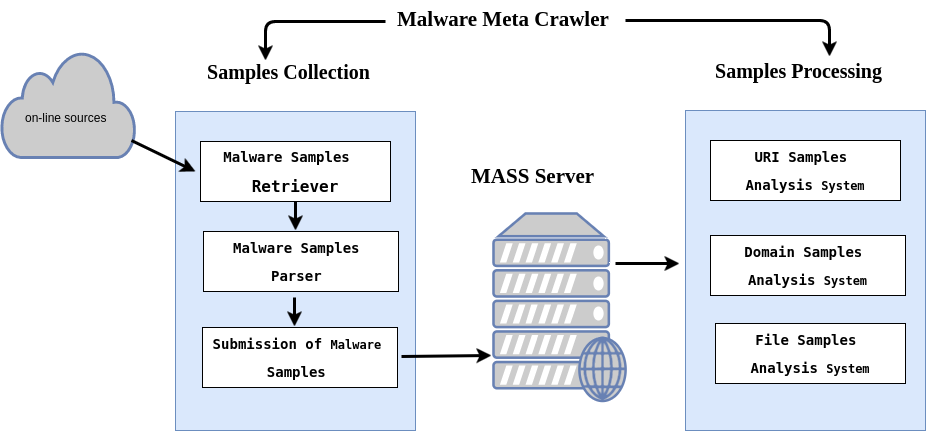
\includegraphics[width=\textwidth, height=.49\textheight]{mass1.png}
     \caption{Generic architecture of the Malware Meta Crawler for MASS System.}
      \label{fig:architecture}
\end{figure}  

\par \textbf{Samples collection:} This subsystem is responsible for the retrieving of malware samples from the different on-line repositories were described the in Section~\ref{sec:sources}. Then the fetched samples are mapped and parsed to the corresponding type (i.e., Domain, URI and File) by this subsystem. Furthermore, 
this subsystem submits the retrieved malware samples  to the MASS server using the MASS API client interface.
\par \textbf{Samples processing:} This subsystem enriches the information of the malware samples retrieved by the sample collection subsystem, also it constructs the relation between the related malware samples. The following are the main modules (i.e., analysis units) of the sample processing subsystem, which automatically receive the new samples submitted to the MASS server:
\begin{itemize}
\item \textbf{URI samples Analysis Client: }this module is responsible to pull the new malware samples of URI type from the MASS server, in order to find the domain of each URI and submit the relation between them to the MASS server.\newline
\item \textbf{File Samples Analysis Client: } this module identify the URI of file samples using predefined regular expression, then it try to download the file from its source and submit it to the MASS server. In addition, it generates the relation between the sample file and origin URI sample.\newline 
\item \textbf{Domain samples Analysis Client: } this module receive all new domain malware samples, then, it looks up for the domain's IP and connect them by the submitting the IP sample and the relation between them to the MASS server.
\end{itemize}

 

\subsection{Process Flow of System} 

This section presents the process flow of the Malware Meta Crawler system that retrieves the malware samples from different on-line sources to  submit them to the MASS server database. Figure~\ref{fig:processflow} illustrates the internal process of the proposed system. 
 

 \begin{figure}[]
  \centering
     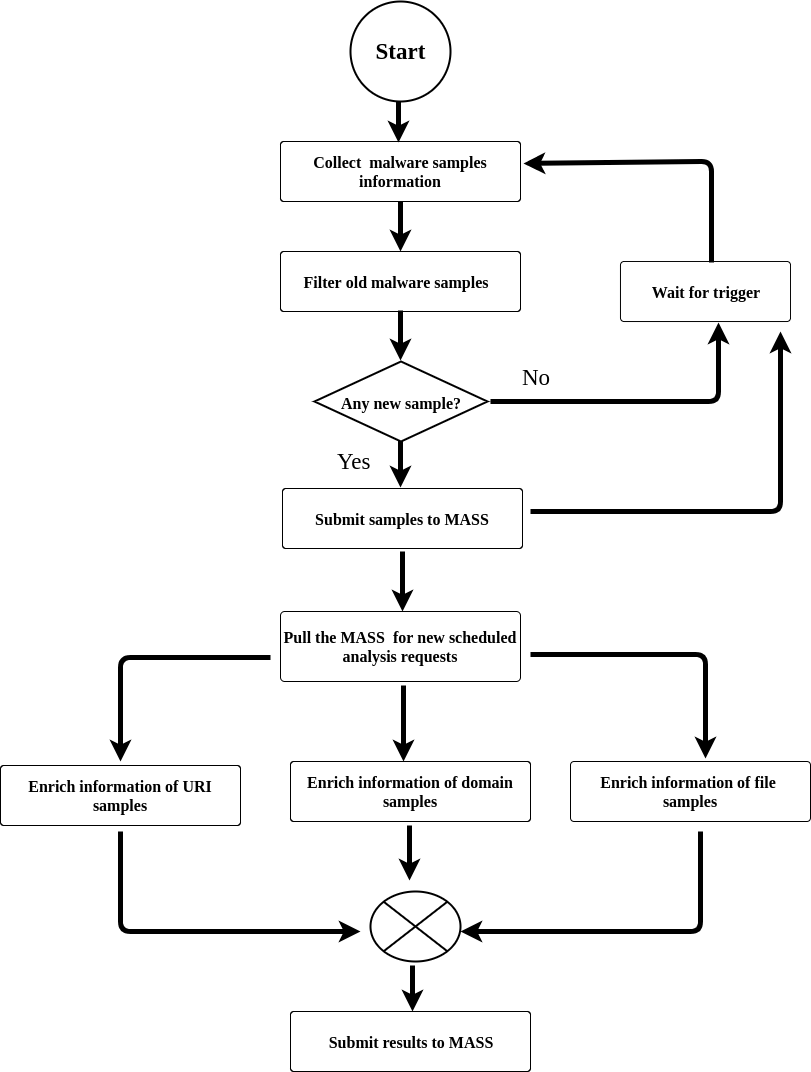
\includegraphics[width=\textwidth, height=\textheight]{mass2.png}
      \caption{Process Flow of Malware Meta Crawler.}
       \label{fig:processflow}
 \end{figure} 


\par  The process begins by collecting the malware samples from the mentioned sources in  Section~\ref{sec:sources}, and these samples include malicious domains and URIs for for infected websites or malware files. The system checks the retrieved samples to filter the old samples were processed and submitted before, and cache information about the  new malware samples in internal storage for later checking. Then the system submits all new malware samples to the MASS server using the offered REST APIs.

\par This process is running again after waiting for the next trigger, which could be automate the execution using cron job  that runs the system after certain  period of time or even manual re-execution. This work flow will continue so that the
system can continuously retrieve the new on-line malware samples.

\par On the other hand, the MASS schedules new analysis requests for the summited new malware samples by the first part of the system's work flow. Then the three analysis clients pull the scheduled analysis requests that contain the information of new malware samples to enrich their information and generate the relation between the related samples. The following are the analysis processes:     

\begin{itemize}
\item \textbf{Enrich information of URI samples}: this process receives all new URI samples to find the URI's domain and submit the relation between the two samples to MASS.

\item \textbf{Enrich information of domain samples}: this process receives all new domain samples in order to look up for the domain's IP and create a relation between them, received domains includes domains submitted by the system from the on-line repositories and the computed domains from previous process (i.e., domains of URI samples).
\item \textbf{Enrich information of URI file samples}: this process receives all new URI samples to filter the URIs that belong to malware files, using a configured regular expression, then the corresponding file is downloaded and pushed to the MASS server. In addition, this process submits a relation between the downloaded file and its original URI. 

\end{itemize}
\section{Details and Implementation}
\label{sec:sec4}
- how the idea + problem is realized + code snippet
- not code docs
This section describes the implementation of the various parts of the Malware Meta Crawler for MASS system.
- don't forget to include the file sample regular expression 
\section{System Evaluation}
\label{sec:sec5}
Evaluation performance + number of samples
- state what do you like to find and how? 
- state perfomance metric like time, memory usage, etc. 
- environment setup 
- present the results 
- conclude findings

   
\section{Conclusion and Future Work}
 \label{sec:sec6}

-briefly sum up what was include/done
-state the overall achievement
-state the future work 
- measure the difference time between submission time between samples. 

 The evaluation of our framework shows that it achieves a comparable
accuracy with respect to some of the best approaches presented in the literature.
\newpage
\begin{thebibliography}{[MT1]}

%

\bibitem[1]{malware_analysis_def} 
Bayer, Ulrich, et al. "Dynamic analysis of malicious code." Journal in Computer Virology 2.1 (2006): 67-77.

\bibitem[2]{worms} 
Kienzle, Darrell M., and Matthew C. Elder. "Recent worms: a survey and trends." Proceedings of the 2003 ACM workshop on Rapid malcode. ACM, 2003.

\bibitem[3]{symantec} 
Symantec. Internet Security Threat Report, Vol. 21 https://www.symantec.com/content/dam/symantec/docs/reports/istr-21-2016-en.pdf, 2016.

\bibitem[4]{malware_analysis} 
Egele, Manuel, et al. "A survey on automated dynamic malware-analysis techniques and tools." ACM Computing Surveys (CSUR) 44.2 (2012): 6.

\bibitem[5]{mass}
The Malware Analysis and Storage System(MASS). URL https://github.com/mass-project/mass\_server/blob/master/README.md.
Accessed: 2017-04-27.

\bibitem[6]{mass_api}
The MASS API Client. URL https://github.com/mass-project/mass\_api\_client.
Accessed: 2017-04-07.

\bibitem[7]{malware_survey}
Manuel Egele. A survey on automated dynamic
malware analysis techniques and tools. ACM
Computing Surveys, to appear.

\bibitem[8]{bot}
Li, Chao, Wei Jiang, and Xin Zou. "Botnet: Survey and case study." innovative computing, information and control (icicic), 2009 fourth international conference on. IEEE, 2009.

\bibitem[9]{virus}
Spafford, Eugene H. "The Internet Worm Incident Technical Report CSD-TR-933." (1991).


\bibitem[10]{maltrieve}
Maltrieve. URL https://github.com/krmaxwell/maltrieve.
Accessed: 2017-04-25.

\bibitem[11]{ragpicker}
Ragpicker. URL https://code.google.com/archive/p/malware-crawler/.
Accessed: 2017-04-25.

\bibitem[12]{python}
Van Rossum, Guido. "Python Programming Language." USENIX Annual Technical Conference. Vol. 41. 2007.
%
\end{thebibliography}

\end{document}